\documentclass{article}

\usepackage{Sweave}
\begin{document}
\Sconcordance{concordance:tutorialJY.tex:tutorialJY.rnw:%
1 2 1 1 0 4 1 1 2 1 0 2 1 5 0 1 1 4 0 2 2 1 0 2 1 5 0 1 1 4 0 2 2 1 0 2 %
1 5 0 1 1 4 0 1 2 2 1}


I will explore the dataset \textbf{mpg} by doing general plots:

\begin{Schunk}
\begin{Sinput}
> library(ggplot2)
> data("mpg")
> head("mpg")
\end{Sinput}
\begin{Soutput}
[1] "mpg"
\end{Soutput}
\begin{Sinput}
> ggplot(mpg,aes(x=displ, y=hwy, colour=cty))+geom_point()+ scale_colour_gradientn(colours = topo.colors(10))
\end{Sinput}
\end{Schunk}
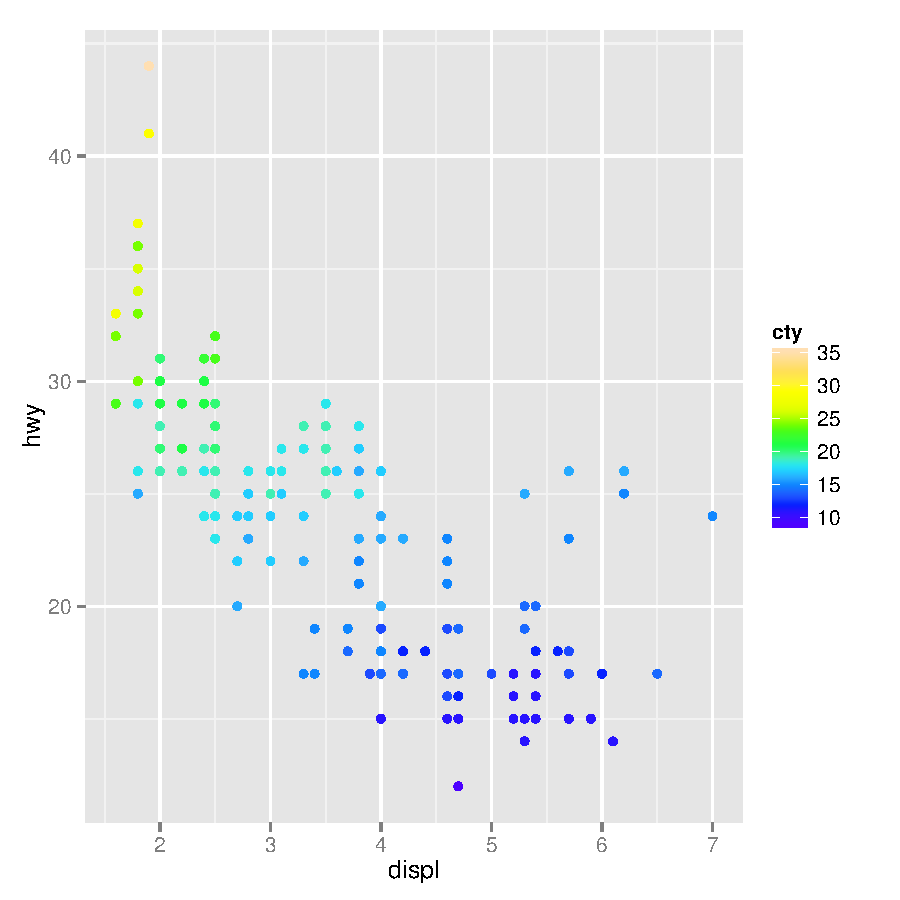
\includegraphics{tutorialJY-Cars1}

\begin{Schunk}
\begin{Sinput}
> library(ggplot2)
> data("mpg")
> head("mpg")
\end{Sinput}
\begin{Soutput}
[1] "mpg"
\end{Soutput}
\begin{Sinput}
> ggplot(mpg,aes(x=displ, y=hwy, colour=drv))+geom_point()+ scale_colour_hue()
\end{Sinput}
\end{Schunk}
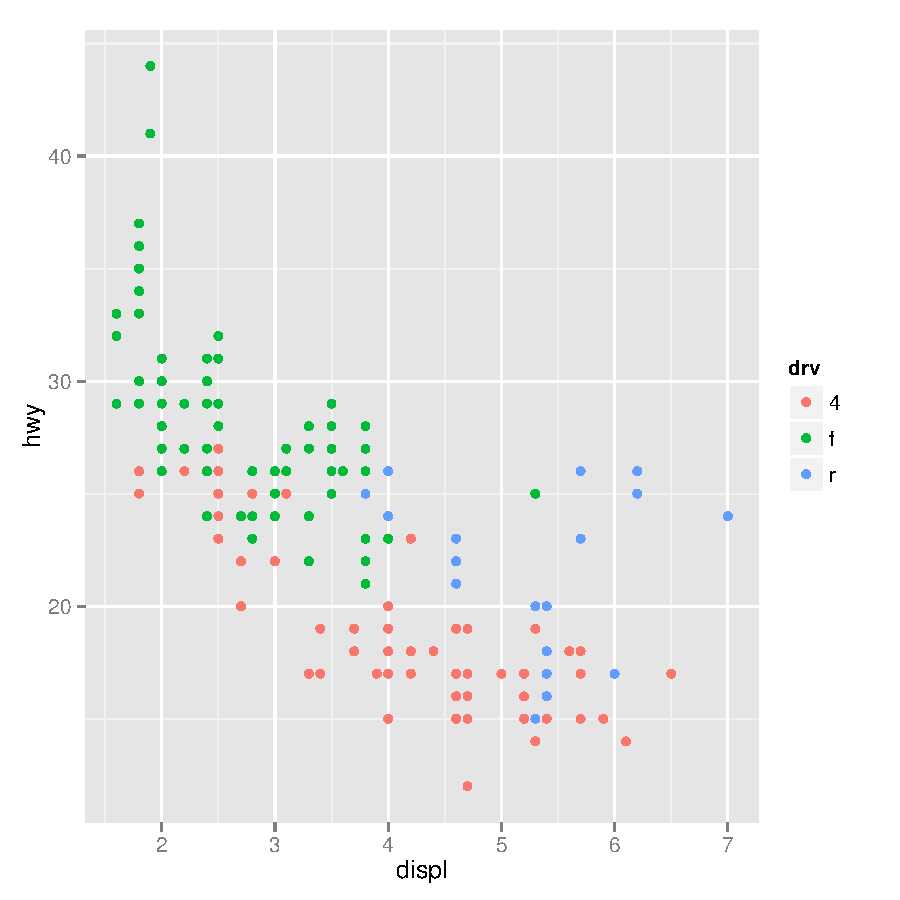
\includegraphics{tutorialJY-Cars2}

\begin{Schunk}
\begin{Sinput}
> library(ggplot2)
> data("mpg")
> head("mpg")
\end{Sinput}
\begin{Soutput}
[1] "mpg"
\end{Soutput}
\begin{Sinput}
> ggplot(mpg,aes(x=hwy, y=cty, colour=displ))+geom_point()+ scale_colour_gradientn(colours = topo.colors(10))
\end{Sinput}
\end{Schunk}
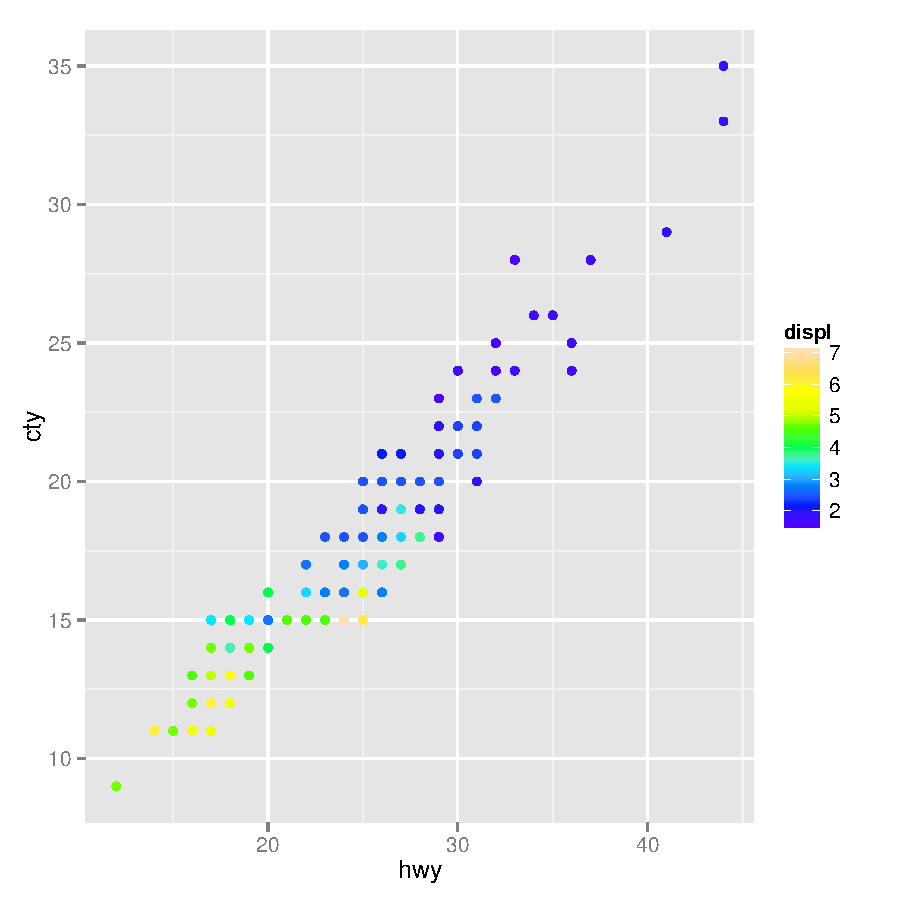
\includegraphics{tutorialJY-Cars3}
This is the end of ggplots.



\end{document}
